\subsection{Passer}
Passer potrebuje chrániť dáta, ktoré sú uložené vo filesystéme iOS. Keďže nechceme, aby používateľ stratil všetky dáta po reštarte aplikácie, potrebujeme ich ukladať mimo aplikáciu (filesystém). Riešením, ako ich chrániť, je šifrovanie. Ak zašifrujeme dáta počas ukladania do súboru, útočník ich nebude môcť rozlúštiť, aj keby sa ku nim dostal. 
Z rôznych dostupných šifrovacích algoritmov sme vybrali 
AES. Táto symetrická šifra používa len jeden kľúč. Pomocou neho šifruje, ale aj dešifruje dáta. Na ukrytie kľúča sme využili architektúru, ktorú obsahujú iPhone smartfóny s technológiou Face ID alebo Touch ID: Secure Enclave.

Secure Enclave (ďalej SE) je špecifický hardvérový komponent telefónu. Má vlastný operačný systém a funguje nezávisle od iOS. Jeho úloha je chrániť citlivé údaje telefónu, najmä kryptografické kľúče. Je používaný na bezpečnostné procedúry ako verifikácia biometrickým odtlačkom \cite{secureenclave} (Touch ID/Face ID). Má vlastný, šifrovaný firmvér, pamäť, disk a šifrovanie na úrovni hardvéru. Tento komponent využijeme na ukrytie AES kľúča. Keďže sa jedná o dve komunikačné strany, musí prebehnúť asymetrická výmena kľúčov, aby si iOS a SE mohli medzi sebou vymieňať dáta bezpečne. 

iOS nekomunikuje s SE priamo. Využíva takzvaný ,,mailbox'' (poštová schránka) systém. Aplikácia umiestni dáta a inštrukcie, čo sa má s nimi vykonať na špeciálne pamäťové miesto (mailbox). Odtiaľ si ich SE vezme, vykoná operácie a výsledok vloží späť do mailboxu, odkiaľ si ich aplikácia vezme. 
\newline
\begin{figure}[H]
  \centering
  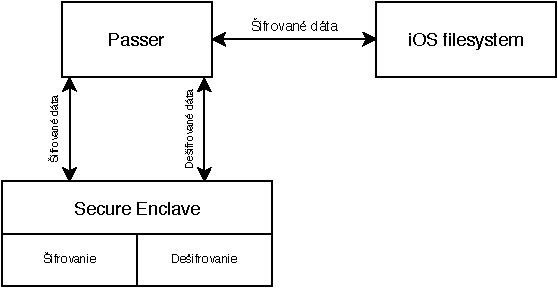
\includegraphics[width=15cm]{img/enclave.pdf}
  \caption{Interakcia Passera s iOS a Secure Enclave.}
  \label{enclave}
\end{figure}

V Secure Enclave vieme vytvárať iba 256 bitové, súkromné kľúče \cite{secureenclave_appledoc}. Tieto kľúče vedia byť použité na Diffie-Hellmanovu výmenu kľúčov na báze eliptických kriviek (ECDH). Výsledok ECDH vieme použiť na symetrické šifrovanie. Tieto kľúče vieme vytvárať výhradne iba v SE. Nie je možné vkladať, či vyberať už existujúce kľúče. Nemožnosť týchto úkonov je základom celej bezpečnosti SE. 

Vytvorenie súkromného kľúča vyzerá v jazyku Swift nasledovne:

\begin{center}
    \texttt{let privateKey = SecKeyCreateRandomKey(attributes as CFDictionary, \&error)}
\end{center}

\noindent Kde \texttt{attributes} je \texttt{dictionary} atribútov súkromného kľúča, kde definujeme jeho vlastnosti (256-bit elliptic curve a pod.). Tento kľúč vytvárame priamo v Secure Enclave. Do premennej \texttt{privateKey} ide iba referencia skutočného kľúča \cite{secureenclave_appledoc}, takže zdroj je uchovaný v SE. Preto nie je možné získať z \texttt{privateKey} jeho dáta, takže tu je bezpečnosť zachovaná. 

Z \texttt{privateKey} vieme získať verejný kľúč a to nasledovne: 

\begin{center}
    \texttt{let publicKey = SecKeyCopyPublicKey(privateKey!)}
\end{center}

\noindent V tomto momente máme vytvorený súkromný aj verejný kľúč, ktorý patrí Secure Enclave. Môžeme začať so šifrovaním.

Symetrické šifrovanie prebieha podľa algoritmu ECIES \cite{ecies}. V kryptografii sa komunikácia medzi dvoma stranami demonštruje ako komunikácia medzi Alicou a Bobom. Bob bude v našom prípade Secure Enclave, Alica bude Passer. Teda:
\begin{itemize}
    \item[-] Bob vlastní súkromný kľúč $x$ a z neho vytvorí verejný kľúč $g^{x}$. 
    \item[-] Alica získa Bobov verejný kľúč $g^{x}$.
    \item[-] Alica vygeneruje súkromný, efemérny kľúč $y$ a z neho verejný, efemérny kľúč $g^{y}$.
    \item[-] Alica vypočíta symetrický kľúč $k$ pomocou key derivation function: $k = KDF(g^{xy})$.
    \item[-] Alica získa šifrovaný text $c$ zo správy m použitím symetrického kľúča $k$ a algoritmu $AES$ nasledovne: $c = AES(k;m)$.
    \item[-] Alica pošle šifrovanú správu spolu s efemérnym kľúčom Bobovi. 
    \item[-] Bob extrahuje z $c$ efemérny verejný kľúč.
    \item[-] Bob vypočíta symetrický kľúč $k$ pomocou key derivation function: $k=KDF(g^{xy})$
    \item[-] Bobov kľúč $k$ je rovnaký, ako Alicin pri šifrovaní.
    \item[-] Bob dešifruje správu $c$ a získa otvorený text: $m = AES(k;c)$.
\end{itemize}

\noindent Zobrazme si tento proces vizuálne. Pri šifrovaní
\begin{figure}[H]
  \centering
  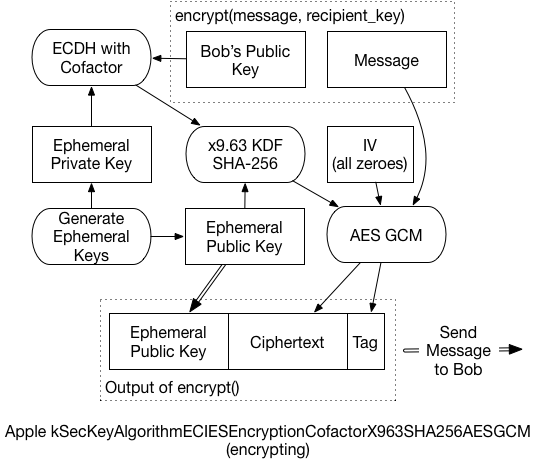
\includegraphics[width=10cm]{img/ecies-arch-encrypt.png}
  \caption{Proces šifrovania podľa algoritmu ECIES.}
  \label{SEencr}
\end{figure}

\noindent vznikajú efemérne kľúče. Efemérny súkromný kľúč spolu s verejným kľúčom patriacim Secure Enclave na základe ECDH vytvoria takzvaný ,,shared secret''. Ten je pomocou KDF zmenený na symetrický kľúč. Kľúč vchádza do AES spolu so správou a inicializačným vektorom. Výsledok je zašifrovaný text spojený s efemérnym verejným kľúčom a tagom. Tento ,,balík'' je odoslaný do SE. 
\begin{figure}[H]
  \centering
  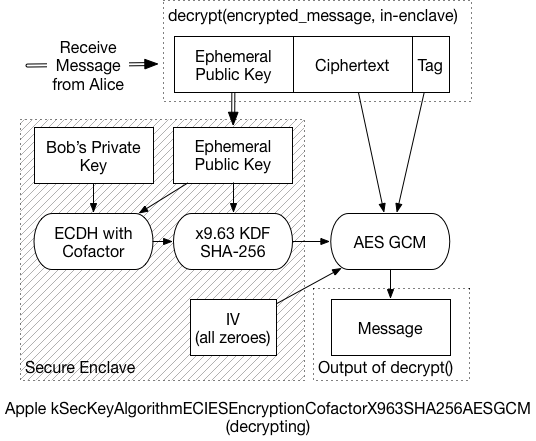
\includegraphics[width=10cm]{img/ecies-arch-decrypt.png}
  \caption{Proces dešifrovania podľa algoritmu ECIES.}
  \label{SEdecr}
\end{figure}

SE spracuje to, čo prišlo. Extrahuje efemérny verejný kľúč. Použije svoj súkromný kľúč a efemérny verejný kľúč na získanie verejného tajomstva. Pomocou KDF získa symetrický kľúč. Ten spolu s inicializačným vektorom, šifrovaným textom a tagom vstupuje do AES. Algoritmus dešifruje text na pôvodnú správu. Jediné, čo SE vráti do mailboxu je táto dešifrovaná správa.

V skratke: pri šifrovaní používame verejný kľúč SE, pri dešifrovaní zase súkromný kľúč SE. Efemérne kľúče sa generujú kvôli dohode o výmene kľúčov (ECDH). 

V zdrojovom kóde Passera existuje trieda \texttt{Vault}. V nej sú všetky položky používateľa počas behu programu: teda, v plaintexte. Po pridaní alebo vymazaní položky sa vo \texttt{Vault} zavolá metóda \texttt{vaultUpdate()}, ktorá vykonáva operácie s dátami. Najprv aktualizuje polia Passer položiek. Potom ich serializuje do JSON štruktúry. Potom túto štruktúru zašifruje pomocou \texttt{vaultEncrypt()}. Táto metóda vracia 
\begin{center}
    \texttt{return SecKeyCreateEncryptedData(publicKey!, algorithm, dataToEncrypt as CFData, \&error) as Data?,}
\end{center}
\begin{sloppypar}
    \noindent čo je zašifrovaný text. Na šifrovanie je použitá vstavaná metóda Swiftu \texttt{SecKeyCreateEncryptedData()}, ktorá ako vstup očakáva verejný kľúč SE, zvolený šifrovaný algoritmus (v našom prípade AES), nezašifrovanú správu (JSON štruktúra s Passer položkami) a smerník na objekt riadenia chýb, ktorý kontroluje chyby a oznámi ich do konzoly v prípade zlyhania. Vrátený zašifrovaný text \texttt{Vault} uloží do filesystému.
\end{sloppypar}

Pri najbližšom spustení aplikácie je najprv od používateľa vyžiadaná biometrická autentizácia. Po úspešnom verifikovaní sa zavolá metóda \texttt{vaultDecrypt()}, ktorá dešifruje dáta a vráti ich: 
\begin{center}
    \texttt{return SecKeyCreateDecryptedData(privateKey!, algorithm, dataToDecrypt! as CFData, \&error) as Data?}
\end{center}
\begin{sloppypar}
    \noindent Metóda \texttt{SecKeyCreateDecryptedData()} očakáva súkromný kľúč SE, zvolený šifrovaný algoritmus (v našom prípade AES), zašifrovanú správu a smerník na objekt riadenia chýb.
\end{sloppypar}

Dáta sú dešifrované. JSON objekt vieme deserializovať a naplniť z neho \texttt{Vault}. Úvodná inicializácia je hotová. Používateľovi sa zobrazí úvodná obrazovka a vidí svoje Passer položky. 

Pri úvodnej biometrickej autentizácii nešlo o šifrovanie/dešifrovanie/výmenu kľúčov. Je to len podmienka k tomu, aby mohlo dešifrovanie vôbec začať. Ak používateľ nemá žiadne položky, tento krok je preskočený. Je zbytočné autentizovať vstup do niečoho, kde nič nie je.
